\documentclass[conference]{IEEEtran}
\IEEEoverridecommandlockouts
% The preceding line is only needed to identify funding in the first footnote. If that is unneeded, please comment it out.
\usepackage{cite}
\usepackage{amsmath,amssymb,amsfonts}
\usepackage{algorithm, algorithmic}
\usepackage{graphicx}
\usepackage{textcomp}
\usepackage{xcolor}
\def\BibTeX{{\rm B\kern-.05em{\sc i\kern-.025em b}\kern-.08em
    T\kern-.1667em\lower.7ex\hbox{E}\kern-.125emX}}
\begin{document}


%%%%%% Think & Fix %%%%
\title{ICE Block: Emergency Contacts\\
\thanks{Columbia University COMS E6181 Advanced Internet Services Fall 2018 by Professor Henning Schulzrinne}
}

\author{\IEEEauthorblockN{Jeongmin Oh}
\IEEEauthorblockA{\textit{M.S. in Computer Engineering} \\
\textit{Columbia University}\\
New York, United States \\
jeongmin.oh@columbia.edu}
}

\maketitle

\begin{abstract}
I present concept and prototype of In Case of Emergency Block(ICE Block),
an Emergency Contacts on Blockchain. Through the ICE Block,
(1) Users can encrypt and store their emergency medical information and contact in Public Blockchain.
(2) Whenever the information are necessary, anyone with a key pair can decrypt and view the information.
(3) It is provided as a service of Public Blockchain, so that anyone can have a copy of the entire Databse,
(4) and the information can be read through the copy even if the internet connection is temporarily impossible.
\end{abstract}


\begin{IEEEkeywords}
Internet Service, Blockchain, Emergency
\end{IEEEkeywords}

\section{Background}
Having more information about patients is crucial to prescribe medical treatments.
If it is possible, medical staffs will be able to treat the patients more accurately and quickly.
However, it is not easy for them to obtain the information without having patient's concent.
In an emergency situation, the problem can be further deepened.
For example, suppose you have a sudden accident at road.
And, Fortunately, someone reported the accident.
First respondents will carry you to the nearest hospital. In bad situation,
they need to follow remote direction from medical staff who is located in remote. What if they are tyring to give an injection when you are in coma?
What if you have a specific response to the injection, or a history of a particular chronic disease they need to know?
If you are lucky, you body doesn't react to emergency prescriptions, or even worse.

We need to save our basic medical information and contacts that is easily accessible by anyone who can help people who is in emergency situation.
There are several solution is available today for this.
First, We can use local storage like cell phone that can show your basic medical information and contact list without unlock it. 
Second, Remote online server can be an alternative.
Third one is leaving physical notes somewhere near us.
All of these solutions have shortcomings and problems that is ICE Block solved.
ICE Block resolves limitations of existing solutions and potentially can be extended its service scope
beyond its original purpose. 

\section{Previous Work}

\subsection{Using Local Storage}
Mobile devices like cell phone provide easy way of saving information in local.
People carry cell phone almost everywhere they go. So, it will be most likely found every accident scene with patients.
Some of the cell phone maker providing functionality of emergency medical information using local storage.
For example, Apple's Medical ID\cite{r1} provide local storage which is available without unlock the device.
Their solution seems pausible but has some limitation.
It is not available when the local storage is not accessible
because of physical damage or no power.
To provide high availability, the information should be stored in remote storage.

\subsection{Using Remote Server}
Some of the goverment provide emergency contact service. Illinois's Emergency Contact Database is good example.
User voluntarily save their information on the database and it can be used in emergency.
I assume their solution built on conventional architecture that is expansive to scale.
Prodiving high reliability with great scalability is burden for any organization.

Using Cloud repository might be a solution but it also has some limitation.
Store and backup a few of line of characters on global cloud service like Goole Docs might be simple and economic solution
but user need to think it will be really available everywhere.
The service may not cross border because there might be political issues.

\section{Design Principle}
ICE Block designed with following requirements withdrawn from previous efforts and requirements.

\paragraph{High Availability}
ICE Block should have High Availability because its service is for human lives. It should minimize service down time which is planned or not. Mobile devices local storage doesn’t meet this requirement because it doesn’t have back up plan when the device is not working. Distributed Database should be considered to meet this requirement.

\paragraph{Sensitive Information}
User provided information should be encrypted so that none of people cannot see their information without the user’s authorization. Symmetric encryption can encrypt and decrypt user information but it doesn’t provide signature functionality. Asymmetric RSA Key meets this requirements.

\paragraph{Low Cost}
Cost of running service should be low enough. Because the services’ nature is for non-profit or civil service. Service architectures and internal algorithm should spend less energy and computational power.

\paragraph{Scalability}
It also needs to provide great scalability. People travels long distance and hard to expect where the accident happen. Providing local service may not cover all emergency. So, it should be not depending on local infra or certain entity.

\subsection{Architecture}
Following the requirements, ICE Block designed as a public blockchain service.
Client can create user’s RSA key pair.
Its public key used as account\_ID.
All information user provided going to be encrypted at client side and then transferred to one of the nodes in the network.
The node accepts the transaction when it has valid signature. See Fig.\,\ref{fig:1}

After receiving transaction, The Server needs to create a new block so that the transactions are linked with existing chain. To create a new block, it needs previous block’s hash and calculated nonce.
Nonce is number of try to find a valid hash that is ending with several zeros. See Fig.\,\ref{fig:2}

The server should consist network with other neighbors. The network selects one chain with algorithm that is agreed by all participants. ICE Block use simple algorithm.
If node found longer than its chain and it is valid, the node replaces its chain with the chain. See Fig.\,\ref{fig:3}
\begin{figure}
    \centering
    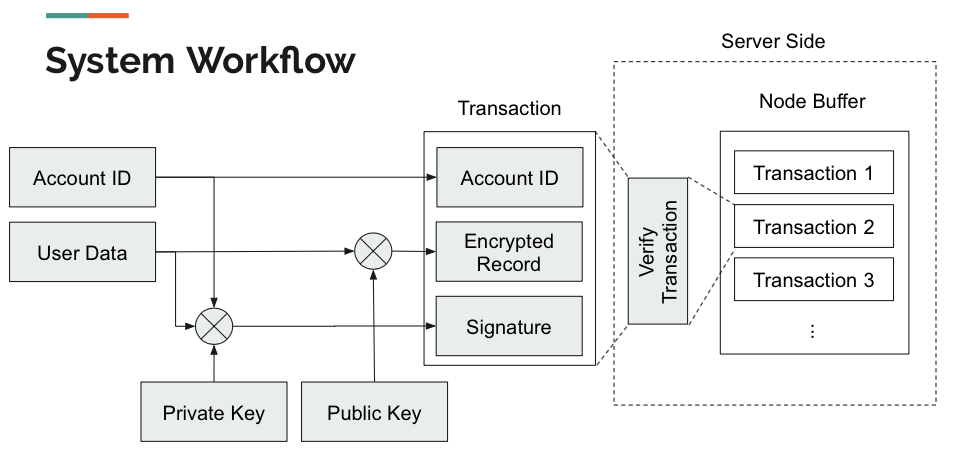
\includegraphics[scale=0.25]{encryption}
    \caption{Creating trasaction}
    \label{fig:1}
\end{figure}

\begin{figure}
    \centering
    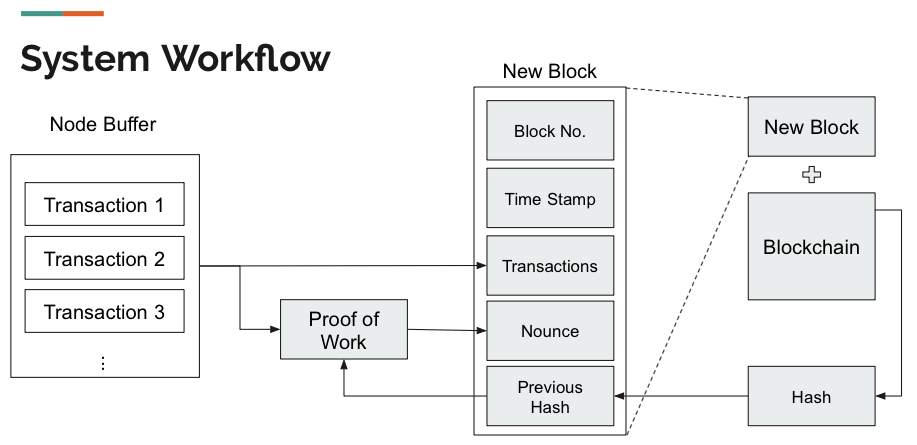
\includegraphics[scale=0.25]{pow}
    \caption{Proof of Work}
    \label{fig:2}
\end{figure}

\begin{figure}
    \centering
    \includegraphics[scale=0.25]{consensus}
    \caption{Consensus}
    \label{fig:3}
\end{figure}


\subsection{Server}
ICE Block Server gets transactions from muliple clients. It needs to validate the transaction and create a new block.
The server also needs to keep data consistancy throughout the network. It use consensus algorithm to select a chain from neighbors.

\paragraph{Validation of Transaction} 
Client send a transaction that is containing account\_ID, encrypted record and signature.
Server needs to validate the transaction whether it is created by owner of private key or not because public key is also used account\_ID in ICE Block.

\begin{algorithm}
    \caption{Algorithm for Validation of Transaction}
    \begin{algorithmic}[1]
        \renewcommand{\algorithmicrequire}{\textbf{Input:}}
        \renewcommand{\algorithmicensure}{\textbf{Output:}}
        \REQUIRE account\_ID, record, signature
        \\ \textit{Initialisation} :
        \STATE validation = \FALSE
        \STATE public\_key = importKey(account\_ID)
        \STATE verifier = PKCS1\_v1\_5.new(public\_key)
        \STATE h = hash(account\_ID, record)
        \\ \textit{Check Validity} :
        \STATE validation = verifier.verify(h, signature)

        \IF{$validation$ $is$ $true$}
            \STATE Push the transaction in the buffer
        \ENDIF

    \end{algorithmic} 
\end{algorithm}

\paragraph{Proof of Work Algorithm}
Every nodes need to prove that they invested some amount of effort to create a new block as nonce.
nonce is number of try the node run hash function to find the hash ending with several cascaded zeros.
Proof of work algorithm prevents divergence of chain with increasing mining difficulty.\cite{r4}

\begin{algorithm}
    \caption{Algorithm for Proof of Work}
    \begin{algorithmic}[1]
        \renewcommand{\algorithmicrequire}{\textbf{Input:}}
        \renewcommand{\algorithmicensure}{\textbf{Output:}}
        \REQUIRE last\_hash, transactions
        \ENSURE nonce
        \\ \textit{Initialisation} :
        \STATE test
        \STATE nonce = 0
        \STATE valid\_proof = \FALSE
        \\ \textit{Loop over to find valid proof} :
        \WHILE{$valid\_proof$ $is$ $false$}
            \STATE guess\_hash = hash(transactions, last\_hash, nonce)
            \STATE nonce += 1
            \IF{$guess\_hash[:difficulty] == '0'*difficulty$}
                \STATE valid\_proof = \TRUE
            \ELSE
                \STATE valid\_proof = \FALSE
            \ENDIF
        \ENDWHILE
        \RETURN $nonce$ 
    \end{algorithmic} 
\end{algorithm}


\paragraph{Conflict Resolution Algorithm}
Server needs to resolve conflict when they add neighbors.
The neighbors may have diffent chain.
Valid and longest chain should be selected in the network.
And every other nodes should update their chain using the chain.
Propagation of the chain in the network is important to keep data integrity.
In my prototype conflict resolution will be excuted when server refresh their view of chain.
It needs to be optimized futher, it is getting whole set of chain from neighbor.
Rathern than sending whole blocks of chain, sending just freshly created block seems more reasonablbe.
Of course checking up whole chain's validity is also important for security reason.

\begin{algorithm}
    \caption{Algorithm for Conflict Resolution}
    \begin{algorithmic}[1]
        \renewcommand{\algorithmicrequire}{\textbf{Input:}}
        \renewcommand{\algorithmicensure}{\textbf{Output:}}
        \REQUIRE neighbors
        \\ \textit{Loop over to find longer chain} :
        \FOR{$neighbor$ $in$ $neighbors$}
            \STATE Get the chain from neighbor
            \IF{$the$ $chain$ $>=$ $self\_chain$ \AND $valid\_chain$}
                \STATE Replace self\_chain with the chain
            \ENDIF
        \ENDFOR
    \end{algorithmic} 
\end{algorithm}


\subsection{Client}
Client provide funtionality of creating pair of public and private key.
public key is used for account\_ID, encryption and signature validation.
private key is used for decryption and sign transaction.
I assume that user can provide the private key when they need it. It might be a type of QRCode or RFID.

\paragraph{Account ID and Password}
Account\_ID is string representation of public key that is also being used for encryption and signature validation.
I chose to RSA 1024 bits to randomly create a key pair. Created binary representation of key pair converted into hexa decimal representation and than decoded using ascii code.
User can create a key pair whenever they need it. 
 
\paragraph{Encryption and Decryption}
Client can encrypt their record that is user provided sensitive information and contact.
To cipher the information, ICE Block use public key that is same as account\_ID.
Decryption works similar way of its reverse order. Client can retrieve encrypted information from the server and use private key to decrypt the information.


\paragraph{Signature}
Technically, Everyone who knows account\_ID can spoil it's records by creating invalid trasactions.
To prevent this problem, ICE Block provides signature that is used in validation algorithm at server side.
I chose to use PKCS1 to create the sign and verification.


\section{Prototype}
I implemented prototype of ICE Block using technology below.

\begin{itemize}
    \item OS: macOS Mojave
    \item Laguage: Python 3.7.0
    \item Virtual Environment: pipenv
    \item Microframework: Flask
    \item Front-end: Bootstrap, jQuery, DataTables
    \item Encryption: PyCrypto(SHA, RSA, PKCS1\_v1\_5)
    \item Testing: Postman, Safari
\end{itemize}

Source code of ICE Block is provided on GitHub.\cite{r3}

\paragraph{Managing Packages}
I used pipenv to create and manage python package.
It provides pacakges in two categories production and development.
The list of package requirement is scripted in Pipfile and Pipfile.lock.
These files are used when user install the packages as a reference.  

\paragraph{Running Program}
Both server and client program runs on localhost using ip address of 127.0.0.1.
And also, get an argument of port using -p flag from command line.
Server use port 5000 and Client use 8080 as default.


\section{Demonstration}
I showed ICE Block's functionality in class demo.
Decryption logic fully functional but it's rendering at web is not implemented.


\section{Experience from prototyping}
Throughout the implementation, I learned something new I didn't know before.

\paragraph{RSA has maximum bytes to encrypt}
When I was tring to encrypt whole information which is user provided,
I realized it is not possble.\cite{r5} I created 1024 bits of key that means it can encrypt 
128 bytes including 11 bytes of padding for PKCS1.
I decided encrypt it's value by value. Increasing number of bits of key is not good solution because ICE Block using public key as ID.
ID had to be short enough to be represneted in QR Code for good recognition.

\paragraph{Hash cares order}
ICE Block gets user input as html form and it is treated in Python dictionary.
After encryption, the information delivered using JSON format.
The problem I was encountred is when creating a Hash for the information.
It had to be ordered so I used Python OrderedDict to construct and re-construct.

\section{Futher Work}
To provide better interface to user, key representation should be considered.
The prototype only shows string representation of Account\_ID and private key.
Better way to representation technology should be applied for this.
QR Code or RFID can be an option. To apply QR Code, User can decide it's visibility
But key should be short enough to be easily scanned.

To provide better scalability, Applying difficulty algorithm should be considered
because if it is too easy, The chain may not be converged.
Notifying new block creation is also should be considered.
I presume asynchronous way of consensus can be helpful.

\section{Conclusions}
ICE Block provide scalable database for emergency contact.
I implemented prototype and showed its service concept in Demo.
It is a light weight public blockchain network anyone can run.
User doesn’t have to worry about lost or damage of their local storage.
And It can be accepted global standard of emergency contact because it will be maintained by participating nodes not the government or organization.
It means that first respondent doesn't have to spend more time to identify patients.
I hope ICE Block save more lives 


\begin{thebibliography}{00}
    \bibitem{r1} Apple's Medical ID\\
    https://support.apple.com/en-us/HT207021
    \bibitem{r2} Illinois's Emergency Contact Database\\
    https://www.cyberdriveillinois.com/departments/drivers/ECD/home.html
    \bibitem{r3} ICE Block GitHub Repository\\
    https://github.com/battlerhythm/iceblock
    \bibitem{r4} Bitcoin: A Peer-to-Peer Electronic Cash System, Satoshi Nakamoto \\
    https://bitcoin.org/bitcoin.pdf
    \bibitem{r5} RSA Maximum bytes to encrypt\\
    https://security.stackexchange.com/questions/33434/rsa-maximum-bytes-to-encrypt-comparison-to-aes-in-terms-of-security



\end{thebibliography}


\end{document}
